\documentclass[preprint]{style}
\pagenumbering{arabic}

\usepackage{paralist}
\usepackage{graphicx}
\usepackage{url}
\usepackage{amsmath}
\usepackage{setspace}
\usepackage{rotating}



% This gets rid of the block of whitespace on the first page
\makeatletter
\let\@copyrightspace\relax
\makeatother


\addtolength{\topmargin}{-.07in}
\addtolength{\textheight}{.07in}

%\addtolength{\oddsidemargin}{-0.08in}
%\addtolength{\evensidemargin}{-0.08in}
%\addtolength{\textwidth}{0.08in}
\setstretch{1.15}

\begin{document}

\title{Medical Concept Extraction}

\numberofauthors{3}
\author{
\alignauthor
Tristan Naumann\\
\affaddr{MIT EECS}
\email{tjn@mit.edu}
\alignauthor
Samantha Ainsley\\
\affaddr{MIT EECS}
\email{ainsley@mit.edu}
\alignauthor
Salman Ahmad\\
\affaddr{MIT EECS}
\email{saahmad@mit.edu}
}

\date{14 December 2012}

\maketitle
\begin{abstract}

This paper presents a system for extracting medical concepts from patient hospital records. Hospitals and medical practices are increasingly switching to electronic medical records--this trend has opened the doors to exciting applications for Natural Language Processing in medicine and biology. One such application is concept extraction: identifying high-level semantic labels in a body of text. Concept extraction on medical records is useful in automating analysis tasks that would otherwise have to be done manually. For example, hospital administrators may want to tabulate what medications are being prescribed the most. Insurance companies may want to ensure that patients receive proper care and are billed accordingly for fraud detection and auditing purposes. Government agencies may be interested in exploring and better understanding public health trends. Automatic concept extraction systems help to streamline such critical yet laborious tasks.

In service of that end, we present an algorithm and system that is capable of classifying words in medical records across four different medically-relevant categories: (1) problems, (2) tests, (3) treatments, and (4) non-medical terms. This is useful not only in granting end users the ability to analyze medical records, but also in supporting other higher-level Natural Language Processing and learning systems. This paper describes the system's design, implementation, and performance when tested on set of 500 pre-annotated medical records from Boston-area hospitals.


\end{abstract}

\section{Introduction}
TODO(SAM):
Lorem ipsum dolor sit amet, consectetur adipisicing elit, sed do eiusmod tempor incididunt ut labore et dolore magna aliqua. Ut enim ad minim veniam, quis nostrud exercitation ullamco laboris nisi ut aliquip ex ea commodo consequat. Duis aute irure dolor in reprehenderit in voluptate velit esse cillum dolore eu fugiat nulla pariatur. Excepteur sint occaecat cupidatat non proident, sunt in culpa qui officia deserunt mollit anim id est laborum.

\section{Background}
TODO(SAM):
\subsection{Related Work}

\subsection{Machine Learning}

Our system addresses the particular challenge of assigning concept labels to terms in medical records, but the task of assigning labels from multiple classes over a set of entries is a classic machine learning problem. Supervised multi-class classification algorithms assign labels to input data entries using a model trained on a data set of pre-labeled observations. There are countless methods that support multi-class classification--for the purpose of this work, we employ three well-known strategies (general Support Vector Machines, linear Support Vector Machines, and Conditional Random Fields) and compare their respective accuracies given our data sets and chosen features (section 4).

\subsubsection{Support Vector Machines}
Support vector machines (SVMs) aim to maximize the margin between decision hyperplanes, which separate training examples in feature space. Training examples are represented as points in feature space that are mapped to create independent classification regions with the largest possible gap between regions. In use, the SVM maps new examples into this space and assigns a label based on the classification region in which the example point resides. 

Often problem sets are not linearly separable in feature space. To overcome this challenge, SVMs often map the original feature space into a higher-dimensional space--the specific mapping defined by a kernel function, which is chosen for efficiency based on the specific classification problem. Separating hyperplanes, which are defined as vectors, can then be chosen as linear combinations of feature vectors in the training set.

We tested a non-linear SVM as provided by the open-source library, LibSVM \cite{libsvm}.

\subsubsection{Linear SVMs}
As mentioned previously, we cannot always expect linearly separable training data. However, for large enough data sets, linear SVMs and SVMs with nonlinear mappings yield similar performance. By eliminating the need for a kernel mapping, training becomes much less costly through use of a linear support vector machine. 

We additionally tested a strictly linear SVM using the open-source library, LibLinear \cite{liblinear}, which provides an L2-loss linear SVM solver.

\subsubsection{Conditional Random Fields}
Conditional random fields (CRF), unlike SVMs, is a probabilistic modeling method. The strength of CRF's in the case of classification for NLP is that it can take neighboring samples (i.e. context) into account when handling individual observations. A CRF is a type of undirected graphical model, which models a conditional probability distribution between observations and output values, which are represented as nodes. Given a sequence of words, this graph takes the form of a chain analogous to a Hidden Markov model. The conditional dependency of each output label on a given input is computed using a feature function in which features are given specific numerical weights and combine to determine the label's likelihood. 

We tested our features using an open-source CRF library, CRFSuite \cite{crfsuite}, in addition to our SVMs.

\section{Challenges}
There are several unique challenges which arise due to the the nature of the dataset and the approach of leveraging traditional machine learning classifiers for natural language.

\subsection{High Dimensionality}
In order to utilize traditional machine learning classifiers for natural language processing, it is necessary to generate linguistic features for each item that requires classification. The linguistic features which characterize each item often do not have a meaningful strict ordering (e.g. it is not meaningful to say ``muffin'' $>$ ``bread'' if your feature was the word itself). Therefore, it is necessary to represent each feature without a strict ordering as a binary dimension reflecting the presence or absence of that feature.

Using this binary dimension representation results in a high dimensional space (e.g. using a word itself as a feature results in a number of dimensions equal to the size of the vocabulary of the training data). Further, the high dimensional space is exceptionally sparse since each item generally only satisfies one binary dimension for the feature. For non-asymptotic cases found in practice, this generally means that the feature space grows much faster than the amount of data and most of the theoretical guarantees of the traditional machine learning algorithms do not hold.

Further, our best intuition often falls short in high dimensional spaces \cite{dimensions}. So it is difficult to generalize the utility of a feature to the entire data set even if it appears to be relevant for a handful of documents.

\subsection{Biased Data}
Many machine learning classifiers assume relatively balanced data with respect to the class labels available. However, in the task of concept extraction it is most often the case that there is a null concept class indicating that the token is part of no relevant concept which is overwhelmingly more abundant than the concepts. The bias of the class labels in the data presents a challenge because a classifier optimized with respect to accuracy will be inclined to simply assign the null concept class for all labels since that will result in relatively high accuracy. Such classifiers will not, however, perform well with respect to more meaningful measures such as precision, recall, or F1-measure.


\subsection{Amount of Data}
As with many statistically-grounded projects, there is often only a limited amount of data available. Within the medical domain this holds particularly true due to the expertise (and subsequent cost) required to provide annotation and the inability to easily merge data from multiple sources -- either due to the differing formats in which it is stored/accessed or various legal restraints in place to protect patients.

Such dearth of training data means that the amount of test data is often much larger than the amount of training data available. Consequently, it is even more difficult to obtain decent results if the models trained even moderately overfit the training data -- a particular risk due to the sparse distribution of high dimensional items discussed previously.

\subsection{Data Usage Agreements}
In addition to limited availability of data, it is often difficult to obtain the data that is relevant. Even for ``open'' data sets such as those provided by the i2b2 National Center for Biomedical Computing, one must sign a data use agreement in order to maintain compliance with the U.S. Health Insurance and Accountability Act (HIPAA) privacy and security rules. The approval process for ``open'' data sets can still take weeks, while access to more controlled data sets can often take months and require security measures such as single physical machine access.

\section{Design}

\subsection{Data Flow \& Classification Task}
Our system considers each document to be a stream of words grouped by sentences, and it attempts to provide the correct concept classification for each word. In order to identify the appropriate concept, our system considers natural language features for each document in successively broader contexts. Specifically, we first consider features using only the word itself as context, next we consider features which span the sentence, and last we consider n-gram features. In the sections that follow we discuss the linguistic features used in each context.

\subsection{Word Features}
Using only the word as context we are able to generate several interesting linguistic features. These features generally take on one of three forms: (1) intrinsic property of the word, (2) binary indicator for properties that we think are interesting, and (3) various techniques that map words into a small dimensional space such as stemming and word shape.

\subsubsection{Word}
The most obvious property of each word is perhaps the word itself. Since there is no linguistically meaningful, strict ordering over words, each word is represented as its own dimension. Consequently adding a baseline feature containing the word increases the dimension of our feature space to the size of the vocabulary in the training data. Nevertheless, the complete word serves as a fruitful feature in medical term classification in which many words carry the same meaning regardless of context. For example, terms such as "x-ray", "screen", "exam", "veal", and "sats" should be consistently recognized as test terms, just as "swelling", "failure", "trauma", and "syndrome" always indicate problems, and "therapy", "anesthesia", "vaccine", and "medication" are treatments. Granted, words like "heart" could be part of "heart rate" or "heart attack" and beg for more generic features.

\subsubsection{Length}
The next most obvious property of each word is its length. Unlike using the word as a feature, there is a strict ordering over length and consequently the addition of this feature increases the dimension of the space by only $1$. While the linguistic merit of length as a feature can be debated in conventional natural language processing, we felt it would play a large role in medical language in order to distinguish treatments, tests, and problems from words without a concept. Intuitively this is because often times treatments in the form of medications consist of long medical names, as do some of the words in medically described problems and tests.

\subsubsection{MIT Regular Expressions}
In order to capture some general characteristics of each word we included a set of regular expressions each of which adds a dimension to our classification. Such features help allow not only to pick up on traits within different medical categories--such as tests which are often abbreviated or contain numbers--but also to easily rule out non-medical terms such as days, phone numbers, etc. The characteristics we chose are as follows:
\begin{itemize}
\item {\tt INITCAP}: first letter is capitalized and alphabetic,
\item {\tt ALLCAPS}: entire word is capitalized and alphabetic,
\item {\tt CAPSMIX}: the word is a mix of capital and lowercase alphabetic characters,
\item {\tt HASDIGIT}: there is a digit in the word,
\item {\tt SINGLEDIGIT}: the token is a single digit,
\item {\tt DOUBLEDIGIT}: the token is a two digits,
\item {\tt FOURDIGITS}: the token is a series of four digits,
\item {\tt NATURALNUM}: the token is a natural number,
\item {\tt REALNUM}: the token is a real number,
\item {\tt ALPHANUM}: the token contains only digits and alphabetic characters,
\item {\tt HASDASH}: the token has a dash,
\item {\tt PUNCTUATION}: the token is punctuation,
\item {\tt PHONE1}: the token is a phone number,
\item {\tt PHONE2}: the token is a phone number with area code,
\item {\tt FIVEDIGIT}: the token is a series of five digits,
\item {\tt NOVOWELS}: the token does not contain vowels (i.e. abbreviations),
\item {\tt HASDASHNUMALPHA}: the token consists of a dash, numbers, and alphabetic characters, 
\item {\tt DATESEPERATOR}: the token is a date separator (e.g. {\tt [-/]})
\end{itemize}


\subsubsection{Porter Stemmer}
We already discussed the benefits of using entire words as features, but similar words come in many different forms. Motivated by generalization, we chose to use word stems as features and approached this feature extraction using three different stemming algorithms--two at the word-level and one at the sentence level (See 5.3.2). The addition of word stem features to our system improved our testing CRF F1 scores from 0.58 to 0.82.

Namely, we used the Porter Stemming Algorithm, as developed by Martin Porter.  This particular stemming algorithm is divided into a number of linear steps. Word letters are first replaced by symbols for vowels, V and consonants, C. The measure, m, of the word is computed as the number of repetitions of the pattern VC, and this is used to determine whether suffixes ought to be removed. Plural word forms, such as  sses $\rightarrow$ ss and removal of trailing s's, are then removed; followed by the removal of past participles; and finally terminal y's are replaced with i's. Subsequent steps handle different orderings of suffices by translating double suffices into a single suffix and then removing suffices under certain predefined conditions.

\subsubsection{Lancaster Stemmer}

Derived from the Porter Stemmer, the Lancaster Stemmer was used to provide a second word stem feature to our system. By constant, this stemming algorithm uses a table of rules that specific the removal or replacement of an ending. Endings are replaced to maintain properly-spelled words throughout the stemming process--this avoids the need for an additional recoding or partial matching phase. 

The rule table looks for the following information about each word: Endings of one or more characters (stored in reverse order); an optional intact flag; a digit specifying the removal total;  an optional append string of one or more characters;  and a continuation symbol. The stemmer first inspects the final letter of a term and considers the first relevant rule in the table. If the rule conditions are not satisfied, another rule is considered, otherwise the rule is applied and the ending is removed or reformed. This process is repeated until a termination symbol is uncovered and the word is presumed to be in its stem form.

\subsubsection{Word Shape}
In the same spirit of our word length and MIT RegEx features, we decided to look at the high-level shapes of individual words for better generalization. More specifically, we encode words into new strings that give a sense of their capitalization and punctuation patterns as well as approximate length. We tested a variety of open-sourced word shape classification methods including two methods written by Dan Klein, one of which simply classifies words as numeric, strictly upper or lower cased, or mixed, and a second, more fine-grained classifier that attempts to group words into equivalence classes by collapsing sequences of the same time. Additionally classifiers developed by Christopher Manning seek to make less distinctions mid-sequence by sorting words based on length. Each word shape classifier result added an additional dimension to our feature space. By naively including all word shape alternatives as features, we were able to improve our testbed CRF F1 score from 0.82 to 0.85.

\subsubsection{Additional Feature Considerations}
The word-level features that we ultimately decided to include in system were chosen based on performance gain, but many others were explored in testing. These features were selected after close examination of our training data, and are worthy of discussion. It is possible, of course, that there is a more optimal feature set than our final choice that includes the features listed below:

\begin{itemize}

\item {\tt Metric Units}
A clear trend we noticed our medical record data was that numbers followed by metric weights (i.e. mg, milligrams, grams) are almost always part of treatment descriptions. Whereas numbers followed by metric lengths or areas are typically part of problem observations. We still believe this could be a useful feature for related systems.
 
\item {\tt Word Endings Indicative of Medical Problem Type}
Another obvious trend specific to medical problems are diseases ending in "itis" such as "bronchitis", "cellulites", "fibrositis", etc. and conditions ending in "ic" such as "diabetic", "anemic", etc. We added a regular expression to flag words with these endings, but the feature did little to nothing to improve performance. Such observations were likely already handled by our other word features.

\item {\tt Prognosis Locations}
Many diagnoses include locational information that should be tagged as part of the problem (i.e. "C4-C5 herniated disks"). We still think that a robust feature of this form could benefit our system, but our particular attempts proved unsuccessful.  

\item {\tt Flag Words}
Certain terms such as those described in 5.2.1 are consistently labeled as "problems", "tests", or "treatments". We attempted to create small dictionaries of these terms and assign flags to words that fall into one of the three dictionaries. The issue with this strategy is that words that words that should be labeled as one of our three medical terms but do not appear in the dictionary are now more closely aligned with purely non-medical words. That said, this feature improved accuracy for our three categories, but also yielded far too many false positives.

\end{itemize}

\subsection{Sentence Features}
Even though the primary goal of our system is to tag concepts at the word level, these individual words often need to be considered in context. Before extracting the word-level features described in 5.2, we first analyze medical records at the sentence level and assign features to our words based on their usage within those sentences.

\subsubsection{Part of Speech}
A fruitful strategy for any concept extractor is to first tag words with labels indicating their Part of Speech in context. In our case, for example, whether an ambiguous term is used as an adjective versus a noun could distinguish it as part of a test rather than a problem. We used the NTLK max entropy Part of Speech Tagger, which is trained on the Penn TreeBank to tag individual sentences. We then iterate over the returned tags and add these as word-level features, adding another dimension to our feature set for each Part of Speech tag.

\subsubsection{WordNet Lemmatizer}
Unlike the Porter Stemmer and the Lancaster Stemmer, which consider words independent of context, the WordNet Lemmatizer requires words to be processed at the sentence level in order to extract their root form. The WordNet Lemmatizer uses the part of speech tags for individual words, which are assign via NLTK as previously mentioned, in conjunction with a subset of tags used for morphology to extract stems from each word. WordNet references a database of word stems, and uses two types of processes to try to convert input strings into a form present in the database. A list of inflectional endings based on the word's syntactic tag is referenced in search of a match that can be detached from the word. An exception list is also referenced in search for an inflected form. WordNet first checks for exceptions and then uses rules for detachment to transform the word--after each transformation the result is referenced against the stem database until a match is eventually found.

\subsubsection{Formatted Text}
When reading through our training data, we noticed that test results are written in a variety of distinct forms that clearly separate these terms from problem or treatment terms. Since test result forms often spent multiple words such was "O2 sat -- 98\%" or "screen was positive". We wrote a series of regular expressions to capture these patterns with the test term as the first term in the sequence. We iterate over each word in the sentence and run our RegEx suite on the inclusive righthand sequence starting from that word. This feature adds only one additional dimension, and improved our CRF F1 test score from .85 to .90 by boosting our test term detection appreciably.

\subsection{N-gram Features}
Although our primary goal is to classify $individual$ words, a single word in a medical record entry is hardly independent from the next.  More specifically, medical concepts can often span more than one word--we may not be interested in detecting these exact spans, but features from certain words provide insight into how to label their neighbors. For example, ambiguous words such as "heart" could precede "rate" or "disease", and making that distinction between test and problem is much easier when we examine the subsequent word in the sentence containing "heart". A neighboring word can serve as an indicator even if it is not part of the same concept span. For example, words like "showed" and its synonyms are non-medical, but tend to follow a test term. Likewise, "rule out" and "history of" tend to precede problems. With this in mind, we observe all features of immediately neighboring words. 

\subsubsection{Previous}
We take a basic approach to context features by considering the immediately preceding word for each individual word. Given a word with the feature set previously described, we simply duplicate each feature with the corresponding value for it's previous neighbor and rename these features $prev\_$<NAME> (e.g. $prev\_$length).  This serves to double the size of our feature space.
\subsubsection{Next}
Likewise, we duplicate the subsequent word features, which are relabeled as $next\_$<NAME>. At this point, our feature space is tripled, but was already quite large--hence, we decided only to consider surrounding words at a bigram level. Nevertheless, this relatively straightforward step brought out CRF F1 testing score up to 0.98.

\subsection{Parameter Tuning}

\begin{figure}
\begin{center}
	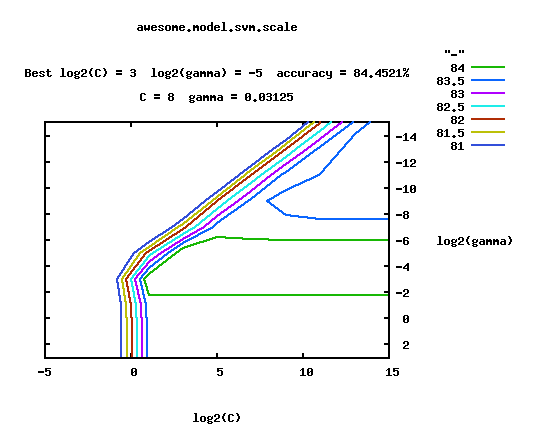
\includegraphics[width=1\columnwidth]{figures/parameter-selection.png}
\end{center}
\caption{An illustration of the grid search process to identify the best parameters values for training the SVM model.}
\label{fig:parameter_selection}
\end{figure}

\begin{itemize}

\item Grid search and grid search image

\item Include that PNG image from easy.py

\item Cross validation

\end{itemize}




\section{System}

\subsection{Code Architecture}

\begin{figure*}
\begin{center}
	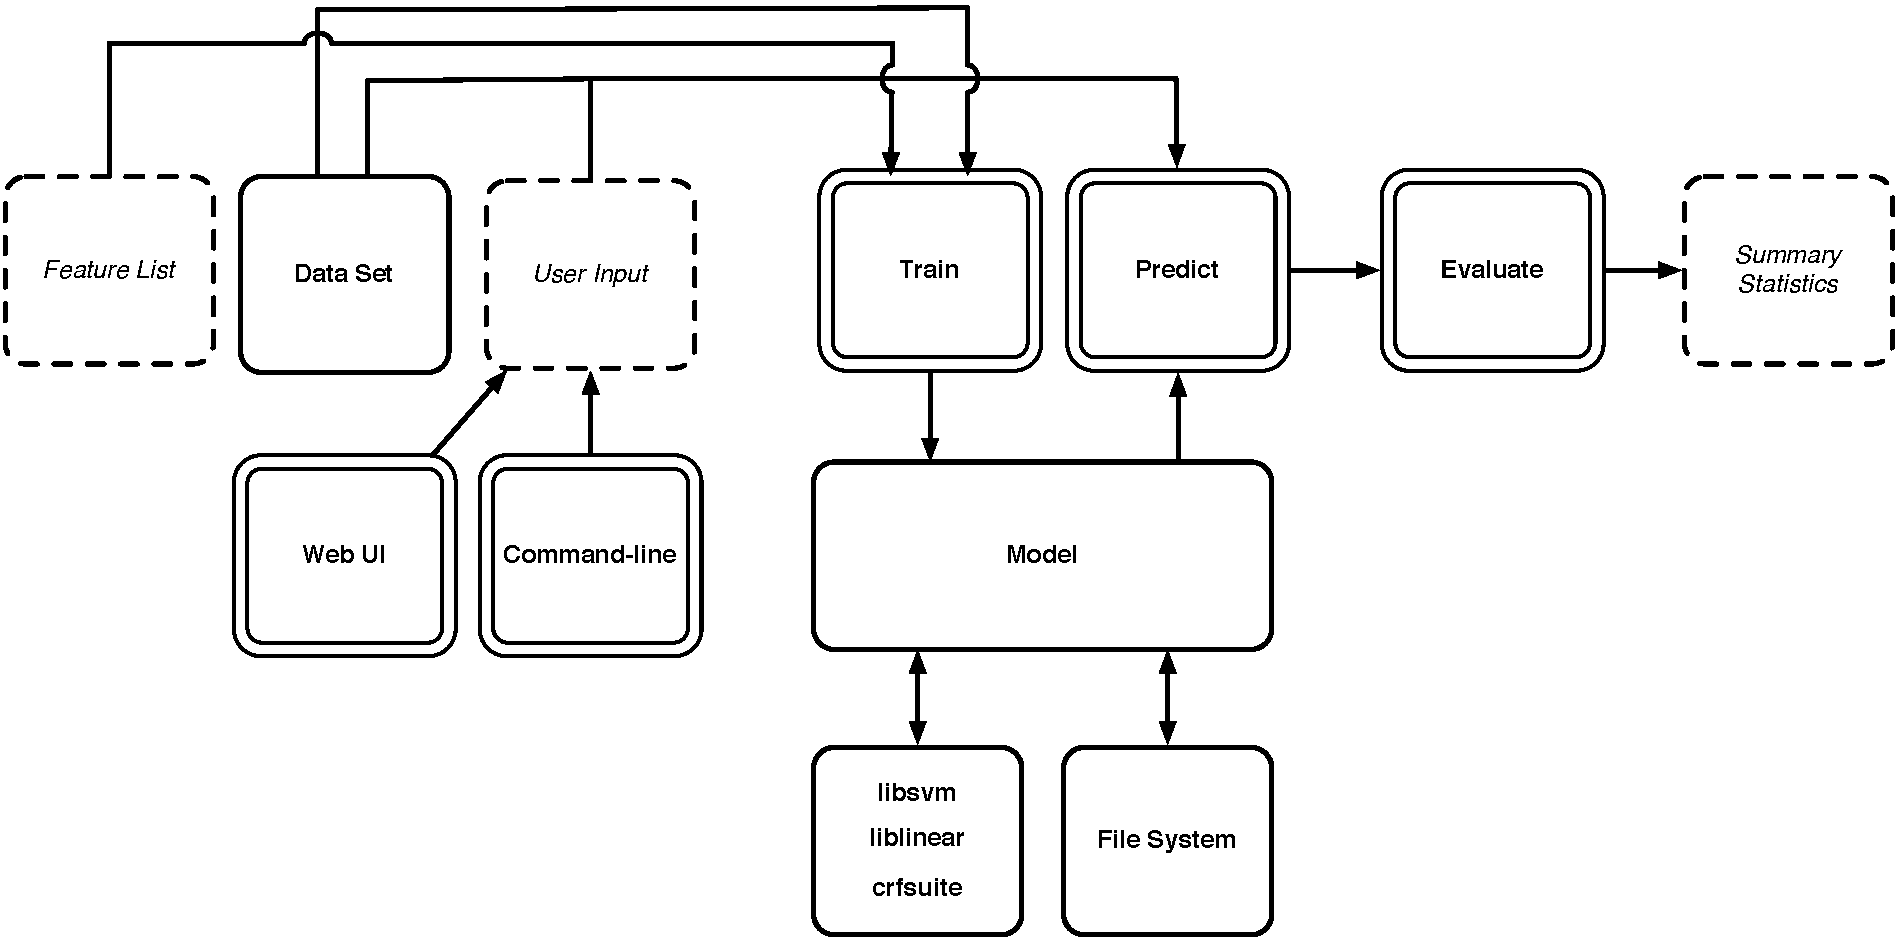
\includegraphics[width=2\columnwidth]{figures/system.pdf}
\end{center}
\caption{An overview of the system and codebase.}
\label{fig:system}
\end{figure*}


We built a fairly comprehensive framework for applying machine learning techniques to NLP domains. We built out a series of useful and reusable library modules and command line utilities to perform various tasks. An overview of the codebase can be seen in Figure~\ref{fig:system} and  all of the code is available online at the following URL:

{\tt https://github.com/tnaumann/ConceptExtraction}.

\subsubsection{Data Formats and File I/O}

Our framework consists of many convenience functions and utilities classes that are designed to perform all necessary file I/O operations formatting output data and parsing input files. There are 3 formats that the code base handles. 

The first format is a straight forward tokenized text file that contains each sentence on a separate line. The test data for training the models were processed into this format. For cases where the sentence was not previously tokenized, the framework utilizes {\tt nltk}'s {\tt sent\_tokenize}  to break a string into sentences and then {\tt nltk}'s {\tt word\_tokenize} to break each sentence into normalized tokens.

The second format is an annotation format that references the tokenized text files and associates a classification label (``problem'', ``tests'', ``treatment'' or ``none'') with spans of words. This format is used in a separate file than the actual input tokenized text file but the two files typically share the same name so we can tell which labels apply to which input. The training and test data sets use this format to represent the ground truth classification of the medical records.

The third and last format is is a sparse matrix format that is utilized by the various command-line utilizes in the code base. Conceptually, the rows in this sparse matrix represent an a single data item (in our case, a single word) that either is a training example or is an input token that needs to a label predicted and the columns represent the various features of that item. The various learning algorithms all use this data format.

\subsubsection{Model Encapsulation and Serialization}

Our framework includes a model class that can be trained on certain data with certain features enabled. The model class supports training a libsvm, liblinear, and crfsuite classifiers that can be used for prediction in the future. One of the nice things, about the model class is that it can be serialized and reloaded dynamically. This is a really nice capability because it allows you to train a large number of models on various subsets of the data and using various different features to see which perform the best.

\subsubsection{Feature Computation}

The framework has a flexible and robust mechanism for computing features on input tokens. Features are implemented as a simple conditional statement in a large {\tt if-else} statement, making it really easy to add new features to the system. Additionally, each model maintains a list of the features that are enabled. Only the enabled features will be executed and computed on the input tokens. Features can be enabled or disabled pragmatically by removing them from the model's feature list. This ability is really important when training models because it enables you to easily explore the impact of certain features and run feature selection.

\subsubsection{Learning Algorithms}

As mentioned previously, the framework's model class has support for training various classifiers: a Support Vector Machine, a CRF, and L2-regularized Support Vector Machine. The implementation of these algorithms is delegates to various third-party libraries described below.

\subsubsection{Data Organization and Directory Structure}


The framework supports a default conventional directory structure to know where to store test, training, and prediction data. This simplifies training new models and testing how well they perform. While these directories can be configured, the defaults are:

\begin{itemize}

\item {\tt data } -  Contains all of the data that is used for training and large testing runs. Again, this is just conventional and it is possible to train and predict on data that is not in this directory. For example, we are able to predict ``one-off-sentences'' as a command-line argument.

\item {\tt data/<data-set-name>/txt } - Contains the raws tokenized text files.

\item {\tt data/<data-set-name>/concept } - Contains the labels that correspond to each of the tokenized files in the ``txt'' directory.

\item {\tt models} - Contains all of the trained models.

\item {\tt models/<model-name>} - Contains the meta data specific to each model that was trained. The framework saves the model's internal state (the features used, the input test set, etc.) as well as the trained parameters for the libsvm, crfsuite, and liblinear classifiers. This information is used to deserialize and load a model at runtime for prediction tasks.

\item {\tt models/<model-name>/predictions/} - Contains output files with the predicted label for each word in the input file.

\end{itemize}

\subsubsection{Command-line Utilities}


The framework contains three useful command line utilities to interact with the system. The functionality provided by these utilities are also exposed by a Python API so other developers can interact with the system natively in their own Python scripts without having to fork calls to the command line. 

\begin{itemize}

\item {\tt train.py } -  Trains a model using the specified training data and output model name.

\item {\tt predict.py } -  Predict the labels for the specified input files and write the labels to a designated file.

\item {\tt evaluate.py } -  Compare the predicted labels to the gold standard labels and print outs the confusion matrix, precision, recall, and F1-scores. 

\end{itemize}


\subsection{Web Service}

In addition to the various command line utilizes described in the previous section our system also includes a Web-based service that allows users to manually input a single sentence, select a model to use for prediction, and see the predicted labels that model generated for the input. Figure~\ref{fig:web_interface} shows a screenshot of the web application in use.

The Web service was written in Python and directly interoperates with the rest of the code base. To run the Web applications simply execute the {\tt web.py} file in the source tree. The Web app allows you to label a sentence using any of the models that we have previously trained. This is useful for spot checking certain sentences and observing how different models behave. The Web app assumes that models have already been trained and placed into ``models'' directory in the source tree. By default, the application will host itself on port 5000. You can also see a live version of the Web service at:

{\tt http://saahmad.media.mit.edu:5000/ }

\begin{figure}[t]
\begin{center}
	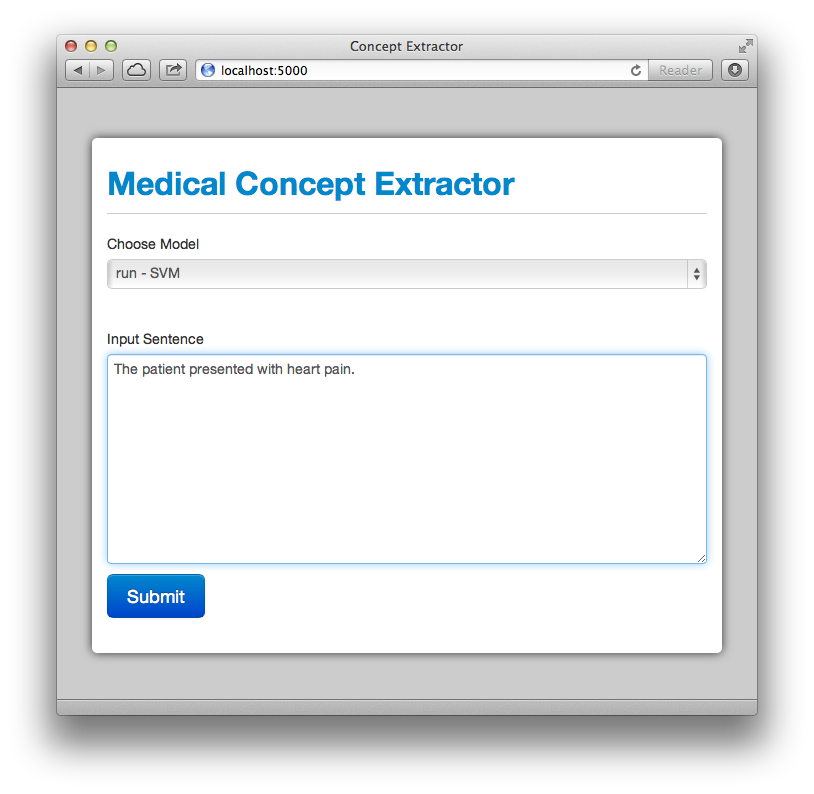
\includegraphics[width=0.75\columnwidth]{figures/web-interface-1.png}
	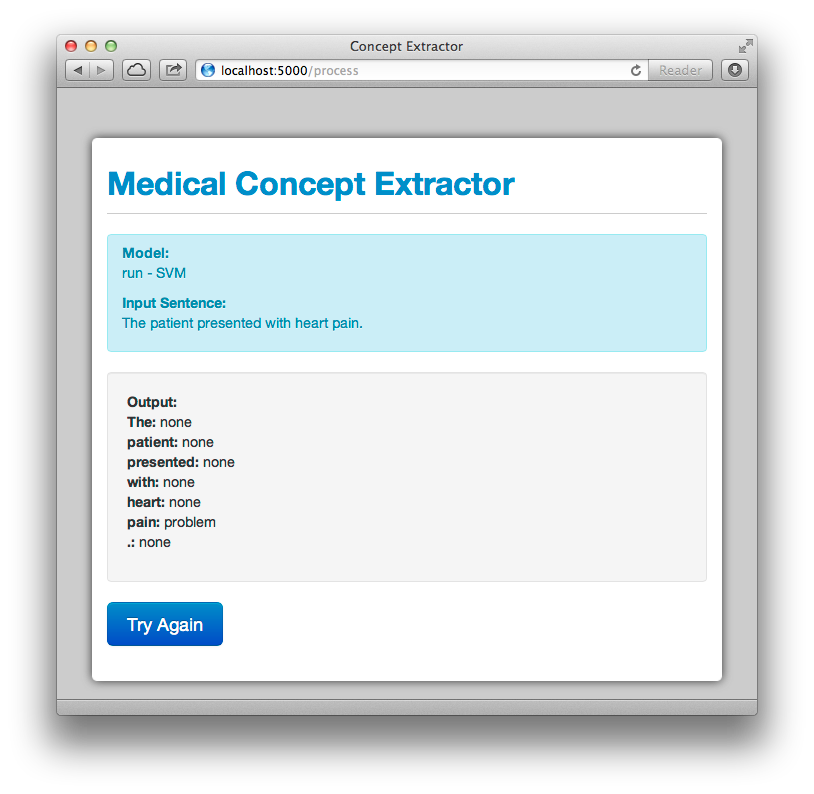
\includegraphics[width=0.75\columnwidth]{figures/web-interface-2.png}
\end{center}
\caption{The Web application interface that allows users to manually input a sentence and have it labeled using one of the previously-trained models. In this case we are using an SVM model that was trained using all of the features.}
\label{fig:web_interface}
\end{figure}


\subsection{Libraries}

Our code leveraged various 3rd party libraries for training the models and generating features. A summary of the libraries that we used is shown in the list below:

\begin{itemize}

\item {\tt libsvm} \cite{libsvm}: libsvm provides a fast implementation of Support Vector Machines. It includes a command line utility that takes a training data (with all of the features formatted in a sparse matrix representation) as input and outputs a SVM model trained on that data. It also includes a command line utility that allows users to specify a desired model and predict the classes on new input. Our code base forks process calls to these utilities to train SVM models, although a lot of the parameter tuning and feature selection is handled elsewhere in our codebase.

\item {\tt liblinear} \cite{liblinear}: liblinear is a linear classifier library that has special support multi-class classification. It also provides easy to use training and predicting command line utilities that accept a similar input format as libsvm.

\item {\tt crfsuite} \cite{crfsuite}: crfsuite is an implementation for conditional random fields and includes command line front ends to train a model on data and to predict the labels on an unseen data set. The data format for the input training files is also a sparse matrix representation but is slightly different from the format used by libsvm and liblinear. Our codebase nicely abstracts out these format differences and produces the right format depending on the model in use.

\item {\tt nltk} \cite{nltk}: nltk is a very popular NLP library written in Python. We leverage nltk to generate some of the features on our data. In particular, we utilize nltk's maximum-entropy part-of-speech tagging as well as many of its stemming algorithms.

\item {\tt flask} \cite{flask}: Flask is a micro Web framework written in Python. It contains a small yet useful set of features that allow developers to easily setup RESTful Web backends and an elegant tempting system to gracefully generate HTML. Flask is used to build the Web service portion of the project.

\end{itemize}
	

\section{Results}

\subsection{Data Set}

\begin{figure}[t]
\begin{center}
\begin{center}
	\begin{tabular}{|l|l|l|}
	\hline
	\multicolumn{3}{|c|}{\bf Training Data Set} \\ \hline
	{\bf Label} & {\bf Count} & {\bf Percentage} \\ \hline
	test & 8492 & 5.7\\ \hline
	none & 114783 & 76.7\\ \hline
	 problem & 17326 & 11.6\\ \hline
	 treatment & 8940 & 6.0\\ \hline
	 {\bf Total} & 149541 & 100\\ \hline
	\end{tabular}
\end{center}

\begin{center}
	\begin{tabular}{|l|l|l|}
	\hline
	\multicolumn{3}{|c|}{\bf Testing Data Set} \\ \hline
	{\bf Label} & {\bf Count} & {\bf Percentage} \\ \hline
	test & 17237 & 6.4\\ \hline
	none & 202438 & 75.8\\ \hline
	 problem & 30276 & 11.3\\ \hline
	 treatment & 17298 & 6.5\\ \hline
	 {\bf Total} & 267249 & 100\\ \hline
	\end{tabular}
\end{center}
\end{center}
\caption{The number of each class the in testing and training data sets.}
\label{fig:data_set_counts}
\end{figure}


Deidentified clinical records used in this research were provided by the i2b2 National Center for Biomedical Computing funded by U54LM008748 and were originally prepared for the Shared Tasks for Challenges in NLP for Clinical Data organized by Dr. Ozlem Uzuner, i2b2 and SUNY. As mentioned before, the data came divided into training and test sets and every word was pre-labeled with the following classes: ``problem'', ``test'', ``treatment'', or ``none''. 

The overall size of the data was 10mb and came from Boston-area hospitals and is subject to data use agreements. The training data consisted of 170 medical records and the test data consisted of 256 medical records. Further, the distribution over labels of the training and test sets is provided in Figure~\ref{fig:data_set_counts}.



\subsection{Trained Models}

Overall we trained a total of 23 models using the entire data set. One model was trained with all of the features. We then trained a set of 11 models in which we removed a single feature as well as 11 models in which we had only one feature enabled. Even  though this is not as complete as a running full feature selection, it will hopefully hint at the most useful features.

Recall that each model contains three different classifiers: libsvm, liblinear, and crfsuite. So, in total we attempted training 69 classifiers. Unfortunately, as discussed later in the paper, the libsvm classifiers took very long to train and most were not finished in time. Consequently, their results are not included in this report. Fortunately we were able to train a single libsvm classifier from a model that had all of the features enabled.  So, all in all the results include the output from 47 classifiers (46 liblinear and crfsuite classifiers and 1 libsvm classifier).

\subsection{Runtime Performance}

We deployed the system on a machine running Ubuntu 11.10 with a QuadCore AMD Opteron processor running a 2.5Ghz and 48GB of ram.

In general training the liblinear and crfsuite classifiers was pretty quick. Each took around an hour to train on the entire training set. However, the libsvm classifier took approximate 6 hours to train on the same data.

In terms of predicting labels for unseen input, all classifiers performed equally well. They each took around 1 hour to label the entire test data set. However, the vast major of time was spent computing features on the input rather than actually running the classifiers.

\subsection{Classification Performance}

\begin{figure}[t]
\begin{center}
	\begin{tabular}{|l|l|l|l|}
	\hline
	\multicolumn{4}{|c|}{\bf crfsuite} \\ \hline
	{\bf Label} & {\bf Precision} & {\bf Recall} & {\bf F1} \\ \hline
	
test & 0.8650 &	0.6857 &	0.7650 \\ \hline
problem & 0.7686 &	0.7492	& 0.7587 \\ \hline
none & 0.9321 & 	0.9637 &	0.9477 \\ \hline
treatment  & 0.7911 &	0.6763 &	0.7292 \\ \hline
	
	\hline
	Average: & 0.7512 &	 0.8537 &	0.7891 \\
	\hline
	\end{tabular}
\end{center}


\begin{center}
	\begin{tabular}{|l|l|l|l|}
	\hline
	\multicolumn{4}{|c|}{\bf liblinear} \\ \hline
	{\bf Label} & {\bf Precision} & {\bf Recall} & {\bf F1} \\ \hline

test  & 0.7908 & 0.8347 & 	0.8122 \\ \hline
problem  & 0.5615 & 	0.9246 &	0.6987 \\ \hline
none  & 0.9784	& 0.8646 &	0.9180 \\ \hline
treatment  & 0.6740 &	0.7908	& 0.7278 \\ \hline

	\hline
	Average: & 0.8392 &	 0.7687  &	0.8001 \\
	\hline
	\end{tabular}
\end{center}
	
	
	
		
\begin{center}	
	\begin{tabular}{|l|l|l|l|}
	\hline
	\multicolumn{4}{|c|}{\bf libsvm} \\ \hline
	{\bf Label} & {\bf Precision} & {\bf Recall} & {\bf F1} \\ \hline

     test & 0.8491 &	0.7392	& 0.7903 \\ \hline
  problem & 0.7603 &	0.7692 &	0.7647 \\ \hline
     none & 0.9395	 & 0.9668	& 0.9529 \\ \hline
treatment & 0.8289 &	0.6365 &	0.7201\\ \hline

	\hline
	Averages: & 0.8444 &	 0.7779  & 	0.8070 \\
	\hline
	\end{tabular}
\end{center}

\caption{Results from a model trained on all of the test data with all of the features enabled.}
\label{fig:all_features_results}
\end{figure}

\begin{figure*}

\begin{center}
	\begin{tabular}{|l|l|l|l|l|l|l|l|l|l|l||l|l|}
	\hline
	\multicolumn{11}{|c||}{\bf Feature Set} & \multicolumn{2}{|c|}{\bf F1 Score}	\\ \hline
		\begin{sideways} length \end{sideways} & 
		\begin{sideways} mitre \end{sideways} & 
		\begin{sideways} next \end{sideways} & 
		\begin{sideways} pos \end{sideways} & 
		\begin{sideways} prev \end{sideways} & 
		\begin{sideways} stem\_lancaster \end{sideways} & 
		\begin{sideways} stem\_porter \end{sideways} & 
		\begin{sideways} stem\_wordnet \end{sideways} & 
		\begin{sideways} test\_result \end{sideways} & 
		\begin{sideways} word \end{sideways} & 
		\begin{sideways} word\_shape \end{sideways} & 
	LIN & CRF	\\ \hline

	\checkmark & & & & & & & & & & & &	\\ \hline
	& \checkmark & & & & & & & & & & &	\\ \hline
	& & \checkmark & & & & & & & & & &	\\ \hline
	& & & \checkmark & & & & & & & & &	\\ \hline
	& & & & \checkmark & & & & & & & &	\\ \hline
	& & & & & \checkmark & & & & & & &	\\ \hline
	& & & & & & \checkmark & & & & & &	\\ \hline
	& & & & & & & \checkmark & & & & &	\\ \hline
	& & & & & & & & \checkmark & & & &	\\ \hline
	& & & & & & & & & \checkmark & & &	\\ \hline
	& & & & & & & & & & \checkmark & &	\\ \hline

\end{tabular}
\end{center}
\caption{A summary of the F1-scores from many different models with different features enabled.}
\label{fig:summary_f1_scores}
\end{figure*}

Overall we found that our system did a good job at predicting labels for medical notes. Figure~\ref{fig:all_features_results} shows summary statistics as well as a confusion matrix of a model that was trained with all the features enabled. The results are broken down so we can see the relative performance of each of the individual classifiers. Overall, the system does very well and achieves an average F1-score of {\bf 0.79}.

As mentioned before, we trained a total of 47 classifiers with different features to get an idea for what features were the most important. A summary of the F1-scores of these classifiers is show in Figure~\ref{fig:summary_f1_scores}.

\section{Discussion}

Talk about what we saw in terms of which was the best feature set and model. 

Be sure to include examples of cool cases where it caught a difficult label

Be sure to include FAILURE cases


We stopped using libsvms.


\section{Conclusion and Future Work}


Found that libsvm was not worth while to use

\subsection{Dimension Collapse}
There are several mechanisms we thought of to to collapse the high dimensional nature of the data. Given unbounded time, we would have liked to try the following.

\begin{itemize}
\item First, we used stemming to add additional features to each word much in the same way that the word feature was created. However, after performing more complete feature selection we would have liked to select the best suited stemmer and used that in place of the word feature.

\item Depending on the stemmer selected, we may have also added a list of stopwords that mapped to a single dimension in order to gain a dimension saving over ``uninteresting'' words.

\item Next, we would have liked to investigate a dramatic reduction by creating a list of all words that are only tagged with the null concept class and mapped them all to a single dimension.
\end{itemize}

While the second approach exhibits only a modest reduction (and may be taken care of automatically by some stemmers), the first and third approaches may allow us to dramatically reduce the dimension of the problem. Our hypothesis is that this will certainly improve the runtime performance, and perhaps the classification performance as well.

\subsection{Feature Selection}
In our work, we performed feature selection in-so-far as we thought of a large number of potential features and then tested their efficacy on a small subset of documents. Further, we generated models from the full set of features as well as each individual feature, and the full set with one held out. While these proved effective for the purposes of analysis, a more exhaustive feature selection is certainly desirable. 

\subsection{Parameter Selection}
Likewise, we experimented with parameter selection for the SVM classifiers over a reduced data set and were able to obtain dramatic increases in classification performance. Due to the already long runtime of training SVM classifiers, it was not feasible to perform any sort of robust parameter selection for these models. However, we expect that doing so would provide additional gains.

\subsection{More Data}

It goes without saying that having more data is always nice. This is particularly true in our case because we were training on a relatively small data set and testing on a considerably larger one. In fact, an interesting avenue for future work is to switch our training and testing data sets so we are training on relatively larger data set.
	
\section{Acknowledgments}

We sincerely thank Dr. Robert Berwick  and Geza Kovacs
for their guidance, help, and support. May the Force be with you,
always.


%%%% May the Flow (Max-Flow, that is) be with you all.

%
% The following two commands are all you need in the
% initial runs of your .tex file to
% produce the bibliography for the citations in your paper.
\bibliographystyle{abbrv}
\bibliography{citations}  % sigproc.bib is the name of the Bibliography in this case

\balancecolumns
% That's all folks!
\end{document}
